\chapterauthor{Christfried H. Focke}{AppFolio}
\chapterauthor{Rob M. Sylvester}{Reltio}

\chapter{Natural Language Processing}

In this chapter we introduce modern NLP libraries, techniques and their applications.
This chapter will focus on deep learning methods and less on computational linguistics that require nuanced knowledge of linguistics.
We explore what it means to represent words and sequences of words with rich numeric representations that are better-suited toward modern computational tasks.
We aim to capture some of these modern fine-tuned representations that are specially catered toward a semantic lexicon for medical language.
\\

\noindent This includes:
\begin{itemize}
\item An introduction into fundamental NLP concepts
\item Bootstrapping techniques to iterate on a dataset in the low-resource setting
\item Storing of a reference dataset in a publicly-accessible location
\item Downloading, caching, loading, splitting, and preprocessing of the data
\item Monitoring the training run:
  \subitem Logging and experiment tracking
  \subitem Learning curves
  \subitem Metrics
\item Hyperparameter tuning, some tricks of the trade
\item Offline evaluation and sanity checking
\end{itemize}
We will keep the discussion focused on tasks in epilepsy, using a running example of SUDEP prediction from electronic medical record (EMR) notes.
Many of the concepts introduced here are very general and are straightforward translations to domains outside of SUDEP prediction, epilepsy, and even NLP.

\section{Introduction to Natural Language Processing}

Natural language processing (NLP) is a field of computer science that deals with the extraction, processing, and understanding of human language.
It is known as the field of computer linguistics, and is a subfield of artificial intelligence.
Common NLP tasks include sentence segmentation, tokenization, part-of-speech tagging, named-entity recognition, parsing, question answering, summarization and classification.

How can we teach a computer to perform these tasks?
The first challenge is that computers, at their core, only understand numbers.
So first we need to think about how words, or more generally text, can be represented with numbers such that we can perform calculations on them.
The numbers should allow the computer to assign meaning to words and their context with other words around it.

There is no perfect way to represent language in this numeric fashion. The best we can do is to capture representations that we feel capture the \textit{syntactic} features of text, as well as \textit{semantic} features of text.
Syntactic information refers to grammatical constructs and the way that words are put together in a language. Semantic information refers to the meaning of this body of text. Such distinctions are fundamental concepts in computer science
and date back to the very foundations of information theory. \cite{shannon48}
Much of this chapter, as well as much of the current work in the field of computational linguistics is centered around finding better and better representations that capture both types of this information.

How do we begin to choose these representations?
Do we choose to represent words, or perhaps individual letters?
Do we choose all the words?
What do we do with punctuation and numbers?

\subsection{Vocabularies and Words}
\label{vocabularies_and_words}
In NLP, the set of unique words in a corpus is called a \textit{vocabulary}. While \textit{the} is the most common word in the English language, it is only one entry in a very large vocabulary table. A rare word like \textit{hemispherectomy} is also one
entry in this table. Both \textit{apple} and \textit{apples} might be separate entries in our vocabulary table. Generally the first step in many NLP systems is defining this vocabulary and the rules behind which words are in this table and which words are not.

The process of splitting text into separate smaller units, in this case words, is known as \textit{tokenization}.
When we run many NLP tasks, we almost always preprocess our text by putting it into one of these tokenizers.
The output tokens, in this case words, are the indexes in our lookup table to different numeric representations that can be understood by a machine.
There are a number of great tokenization libraries that are open source, and you should always use them rather than try to implement this yourself.

\begin{python}
  # Example 1: Spacy Tokenization Using Medical Words

  import spacy
  sample = "After a temporal lobe resection, the " \
           "atonic and clonic seizure frequency " \
           "fell by 50%."

  nlp = spacy.load("en_core_web_sm")
  english_vocab = set(nlp.vocab.strings)
  spacy_document = nlp(sample)

  for token in spacy_document:
      found = token.text in english_vocab

      print("{}: {}".format(token.text, found))
\end{python}

The discrete numeric entities created in Example 1 are the indexes for our representations.
The tokenizer system did much of the magic under the hood, lowercasing and standardizing text and creating special tokens for punctuation and numbers.

When we build a vocabulary $V$, we define a preset vocabulary size $|V|$. There is a tradeoff in your choice of $|V|$.
If you choose a number that is too small, then your system will only recognize a few words and lose a lot of important task-specific vocaublary.
However, if you include the entire english language, your system will be slow, expensive, and not perform as well.
Commonly this number is set around 20,000 - 40,000 words in English, though it can be much larger.

Often a vocabulary will include special tokens that make our lives easier when working with NLP tasks.
Common special tokens include:
\begin{itemize}
  \item \pythoninline{[EOS]} - An end of sentence/input marker.
  \item \pythoninline{[PAD]} - Special inputs to ignore, usually following an EOS marker.
  \item \pythoninline{[SEP]} - A separator, which can be used in inputs that contain multiple sentences or samples.
  \item \pythoninline{[OOV]} - Out of vocabulary, also commonly represented as [UNK] (unknown), which is used when we come across a word that does not exist in our vocabulary.
\end{itemize}

The out-of-vocabulary token is of particular importance in medicine. If we load a vocabulary with 30,000 words, often these are roughly the most common 30,000 words in the English language. We will still have a few [OOV] tokens
for rare words. However, just because a general system chooses its vocabulary based on word frequency does not mean that this is the best choice of vocabulary for the task at hand. Medical corpora have a very different word frequency
distribution than non-medical corpora, particulary because of nuanced vocabulary that is absolutely crucial.

%TODO - add some epilepsy-themed example that throws away all the epilepsy words%

In Example 1 above, notice the importance of the words that have been thrown away. If this sentence were to be loaded into a machine as-is, we might be losing far too much information because we have to nearly all of the relevant terminology with OOV tokens.
We will address this issue in the ensuing sections. For now, suffice it to say that we should make sure our vocabularies are catered toward our task at hand or are built in such a way that they can still extract signal from these tokens. Furthermore, we should always sanity check our sample token outputs against our raw text inputs.

\subsection{Word Representations}

Given that we have defined a vocabulary $V$ of words, these are the keys to our lookup table of numeric representations. But what do we store in that table as the value?

A simple way to achieve this representation for $V$ is to assign each word a unique integer $i$.
The word is then represented as a vector $w$ of length $|V|$ with all zeros and a one\footnote{This is also known as a one-hot encoding}. at index $i$.

\begin{python}
  have = [1, 0, 0, 0, 0, 0, ... 0]
  a    = [0, 1, 0, 0, 0, 0, ... 0]
  good = [0, 0, 1, 0, 0, 0, ... 0]
  day  = [0, 0, 0, 1, 0, 0, ... 0]
  ...
\end{python}

We could now represent a sentence as the sum of the word vectors $S = \sum_j w_j$. This representation is suitable as input for any classification algorithm (such as logistic regression or a decision tree), to make a prediction about our target variable, e.g. whether the sentence is relevant to our epilepsy task.
This simple representation fulfills our requirements but comes with some drawbacks:
\begin{itemize}
    \item We implicitly assume that each word in the sentence is equally important.
    \item Each word is equally similar to every other word (e.g. by taking the Euclidean distance between word vectors).
    \item The representation is invariant to a reordering of the words.
\end{itemize}
The first point is a problem, because as we add more word vectors together, the sentence representation will converge to the global average and drown out any signal relevant to the specific sentence at hand.
To address this we can instead write a weighted sum $S = \sum_j \lambda_j w_j$, where each word vector is weighted by its importance $\lambda_j$. There are statistical methods we can use to compute an importance value\footnote{TF-IDF}.
For example a word like \textit{the} is very common and appears in many different contexts.
It is unlikely that there is a lot of signal we can extract from it.
On the other hand, a word like \textit{epilepsy} will be much more rare and specific to a given task, and we would like to raise its importance.
This has the net effect of allowing us to find good representations for larger word sequences.
To address the second point, we will give a brief introduction into Deep Learning (DL) and the extremely powerful concept of \textit{Embeddings}, one that is not only relevant in NLP, but in the world of AI in general.

\section{Deep Learning}
Deep neural networks (DNNs) have revolutionized the field of NLP along with many others. NLP has seen three main architectures emerge over time: fully connected neural networks (FCNN), recurrent neural networks (RNNs), and Transformers.

\subsection{Fully Connected Neural Networks}
FCNNs are the simplest form of neural networks and are characterized by their feedforward structure, where the input is mapped to one or more output nodes, and with an adjustable number of hidden layers in between.
Each node is connected to every other node in the previous and following layer, via a linear transformation (i.e. a matrix multiplication) followed by a non-linear activation function (e.g. a sigmoid).
The addition of a non-linear activation function allows for the capture of non-linear relationships between the input and output, without it the transformation could be rewritten as just a single matrix multiplication.
The key advantage of DNNs is their ability to automatically learn complex representations of the input data using multiple hidden layers, allowing for the capture of high-level features that could not be easily hand-engineered.

While glossing over some details, training any type of DNN can summarized in the following steps:
\begin{enumerate}
    \item Prepare data pairs $(x_i, y_i)$, where $x_i$ is an input sample, and $y_i$ is the desired output
    \item Determine a function $f$, such that $f(\theta, x_i) = \hat{y}_i \approx y_i$, where $\theta$ are model parameters and $f$ is the model architecture
    \item Define a loss function $L(\theta) = \sum_i L(\hat{y}_i, y_i)$ that measures how close the model's output is to the desired output
    \item Optimize $\theta$ to minimize $L(\theta)$
\end{enumerate}


\begin{figure}[h]
    \begin{tikzpicture}
    % Input nodes
    \node[draw, circle] (input1) at (0, 0) {$x_1$};
    \node[draw, circle, below=of input1] (input2) {$x_2$};
    \node[draw, circle, below=of input2] (input3) {$x_3$};

    % Output node
    \node[draw, circle, right=3cm of input2] (output) {$y$};

    % Hidden layer nodes
    \node[draw, circle, right=1.5cm of input1] (hidden1) {};
    \node[draw, circle, right=1.5cm of input2] (hidden2) {};
    \node[draw, circle, right=1.5cm of input3] (hidden3) {};

    % Connect input nodes to hidden layer nodes
    \draw[-Stealth] (input1) -- (hidden1) node[midway, above] {$\theta_{11}$};
    \draw[-Stealth] (input1) -- (hidden2) node[midway, above] {$\theta_{12}$};
    \draw[-Stealth] (input1) -- (hidden3) node[midway, above] {$\theta_{13}$};

    \draw[-Stealth] (input2) -- (hidden1) node[midway, above] {$\theta_{21}$};
    \draw[-Stealth] (input2) -- (hidden2) node[midway, above] {$\theta_{22}$};
    \draw[-Stealth] (input2) -- (hidden3) node[midway, above] {$\theta_{23}$};

    \draw[-Stealth] (input3) -- (hidden1) node[midway, above] {$\theta_{31}$};
    \draw[-Stealth] (input3) -- (hidden2) node[midway, above] {$\theta_{32}$};
    \draw[-Stealth] (input3) -- (hidden3) node[midway, above] {$\theta_{33}$};

    % Connect hidden layer nodes to output node
    \draw[-Stealth] (hidden1) -- (output) node[midway, above] {$\theta_{o1}$};
    \draw[-Stealth] (hidden2) -- (output) node[midway, above] {$\theta_{o2}$};
    \draw[-Stealth] (hidden3) -- (output) node[midway, above] {$\theta_{o3}$};

    % Add labels for input, hidden, and output layers
    \node[left=0.5cm of input1] {Inputs};
    \node[above=0.5cm of hidden1] {Hidden layer};
    \node[right=0.5cm of output] {Output};
  \end{tikzpicture}

    \caption{Generic architecture of a fully connected neural network. The input is mapped to the output via a series of linear transformations and non-linear activation functions. The number of hidden layers and the number of nodes in each layer are hyperparameters that can be tuned.}
    \label{fig:model_architecture}
\end{figure}

\begin{figure}[h]
    \begin{tikzpicture}[
    declare function={f(\x)=\x*\x*\x - 2*\x*\x + 1.5;},
    declare function={fd(\x)=3*\x*\x - 4*\x;} % derivative of f
  ]
  \begin{axis}[
    axis lines=middle,
    xlabel={$\theta$},
    ylabel={Loss},
    domain=0:2,
    ymin=0,
    ymax=1.7,
    samples=100,
    ytick=\empty,
    xtick=\empty,
    xlabel style={below=3mm,font=\large},
    ylabel style={left=3mm,font=\large},
    xtick={0,0.25,0.5,0.75,1,1.25,1.5,1.75},
    ytick={0, 0.5, 1, 1.5},
    xticklabels={},
    yticklabels={}
  ]
  \addplot [blue, thick] {f(x)};
  \foreach \X in {0.1,0.15,...,0.5} {
     \edef\temp{\noexpand\draw [red, -latex, line width=0.7pt] (axis cs:\X,{f(\X)}) -- (axis cs:{\X-0.1*fd(\X)},{f(\X-0.1*fd(\X))});}
     \temp
  }
  \end{axis}
  \end{tikzpicture}

    \caption{To minimize the loss function we need to adjust the parameters $\theta$ in the direction of the steepest descent, which can be calculated by taking the derivative of the loss function with respect to the parameter.}
    \label{fig:loss}
\end{figure}
Here the loss function can take on many forms, depending on the training task, we summarize some of the most common ones in Table \ref{table:losses}.
\begin{table}
    \centering
    \renewcommand{\arraystretch}{1.3}
    \begin{tabular}{|c| c| c|}
    Loss Name & Function \\[0.5ex] \hline
    Mean Squared Error & $\begin{array} {lcl} \frac{1}{N} \sum_{i=1}^N|\hat{y}_i - y_i|^2\end{array}$  \\ [0.5ex]
    Binary Cross Entropy & $\begin{array} {r@{}l@{}} -\frac{1}{N} \sum_{i=1}^N (y_i \cdot log(\hat{y}_i) + (1 - y_i) \cdot log(1-\hat{y}_i)) \end{array}$ \\ [0.5ex]
    Cross Entropy & $\begin{array} {r@{}l@{}} -\frac{1}{N} \sum_{i=1}^N y_i \cdot log(\hat{y}_i) \end{array}$ \\ [0.5ex]
    \end{tabular}
    \caption{Most common loss functions used for various ML tasks. Mean Squared Error is used for regression tasks, Binary Cross Entropy for binary classification, and Cross Entropy for multi-class classification.}
    \label{table:losses}
\end{table}
Training is then formulated as the task of finding the parameter configuration that minimizes the loss function.
We visualize the loss function of just a single parameter in Fig. \ref{fig:loss}.
In order to move towards the global minimum we need to update the parameters in the direction of the steepest descent, which can be calculated by taking the derivative of the loss function with respect to the parameter.
Parameters in the last layer are then updated according to the following rule until convergence
\begin{equation}
    \label{eq:optimization}
    \theta \rightarrow \theta - \alpha \frac{\partial L}{\partial \theta}
\end{equation}
where $\alpha$ is called the \textit{learning rate} and determines the step size, the partial derivative of the loss function with respect to the parameters is called the \textit{gradient}.
Consequently the algorithm is called \textit{Gradient Descent} and is the workhorse of all modern deep learning.
The algorithm trivially extends to the case of multiple parameters in the last layer.
A similar rule applies to parameters in the hidden layers.
Once the gradients of the subsequent layer have been computed we can apply the chain rule from calculus to compute the gradients of the parameters in the current layer -- this is called \textit{Backpropagation}\footnote{Backpropagation}.
% \footnote{https://en.wikipedia.org/wiki/Backpropagation}.

Simple FCNNs have several limitations in NLP.
For example, it is difficult to capture the sequential structure of text data, and they do not scale well to large vocabularies.
Remember, that in order to represent a word in a FCNN, we need to have a one-hot vector of size $|V|$.
To represent a sentence of length $n$, we need to have $n$ vectors of size $|V|$, which is a lot of parameters.

\subsection{Recurrent Neural Networks}
To overcome this, RNNs were introduced.
RNNs are a type of neural network that have loops in their structure, allowing information to flow both forward and backward through the network.
The idea is that we can use the output of the previous step as input to the current step, and the output of the current step as input to the next step and so on.
To encode the meaning of a sentence or paragraph, the model reads the tokens one by one, updating the representation in the hidden state, which can then be used for subsequent predictions.
This allows us to reuse a large part of the parameters, which is crucial for efficient training.
It also means that this architecture is suitable to varying length inputs, as we can stop reading the input once we reach the end of the sentence, which is in contrast to FCNNs, where we have to define the maximum length of the input in advance.
However, this comes at a cost.

For the purpose of training this architecture, you can think of unrolling the network into a sequence of layers, where each layer is a single step in the sequence.
This quickly leads to very deep neural networks, which tend to be difficult to train because the training signal has to flow through each layer.
This is related to a common problem in DL that is known as \textit{vanishing gradients}\footnote{Vanishing gradient problem}
%\footnote{\url{https://en.wikipedia.org/wiki/Vanishing_gradient_problem}}.
It occurs when the gradients used to update the network's parameters become extremely small, a consequence of the backpropagation algorithm where gradients are multiplied by the derivate of the activation function of the subsequent layer.
In the case of a $sigmoid$ its derivative is smaller than one, so that this factor decays exponentially in the number of layers.
This means that the maximum sequence length that can be learned is strongly limited.
There are some workarounds, such as using different activation functions\footnote{$tanh$, $ReLU$} or gating mechanisms\footnote{Long Short-Term Memory (LSTM)}\footnote{Gated Recurrent Units (GRU)} to allow the information to propagate more freely through the network.
But even then, the maximum achievable sequence length is limited to about 100 tokens before the network "forgets" what happens at the beginning.

Lastly, RNNs are inherently sequential because the output of a step depends on the output of the previous step, and vice versa during backpropagation.
We can not parallelize this process making parameter updates, and therefore scaling to large datasets, as well as inference very slow.

\subsubsection*{Attention}
One way to address the vanishing gradient problem is to use a so called attention mechanisms.\cite{https://doi.org/10.48550/arxiv.1409.0473}
The intuition behind them is to assign a weight to each part of the input sequence, indicating the importance of that part for the current task.
These weights are computed dynamically for each step in the processing of the input sequence and allow the model to focus on the most relevant parts of the sequence.

They are implemented as additional layers in the model that calculate the attention weights using a set of learnable parameters and use these weights to weight the hidden states of the RNN at each step in the processing of the input sequence.
The weighted hidden states are then combined and passed through a feedforward neural network to produce the final output.

There are several different types of attention mechanisms, including additive attention, multiplicative attention, and self-attention. Each of these mechanisms has its own strengths and weaknesses, and the choice of mechanism to use depends on the specific requirements of the task and the nature of the input data.


\subsection{Transformers}
The development of attention mechanisms in RNNs laid the foundation for the development of the Transformer architecture, which is now the state-of-the-art in many natural language processing tasks.

The main drawback of attention mechanisms in RNNs is that they require sequential processing of the input sequence, which can be slow and inefficient for long sequences, and doesn't scale to large datasets.
The Transformer architecture was introduced as a solution, as it uses self-attention mechanisms to allow for parallel processing of the entire sequence.

Self-attention works by first embedding the input sequence into a continuous vector space. Then, for each position in the input sequence, the model calculates a set of attention scores, which indicate the degree of dependence between that position and all other positions in the sequence. These attention scores are used to compute a weighted sum of the input representations, which is then used as the input to the next layer of the model.
It is called self-attention because the model is able to put the representations of each token into context of all surrounding tokens (see Fig. \ref{fig:self-attention}).

Each token is assigned an embedding which is multiplied with three trainable weight matrices to obtain three vectors, called Queries, Keys, and Values.
The model first computes the dot product of the Query vector with each of the Key vectors, and then applies a softmax function to the resulting vector to obtain attention scores that are between 0 and 1 and sum to 1, where the softmax function is defined as:
\begin{equation}
    \text{softmax}(x_i) = \frac{e^{x_i}}{\sum_{j=1}^{n} e^{x_j}}
\end{equation}
Finally, the resulting vector of attention scores (Fig. \ref{fig:self-attention}) for each token is multiplied with the Value vectors to obtain the representation for this token.
The outputs of the self-attention mechanism are then passed through a feedforward neural network to produce the output of a so called \textit{encoder block}.
Many such encoder blocks are stacked on top of each other to form the encoder of the Transformer architecture.
In some architectures one wants to generate new text, for which we need a \textit{decoder}.
It has a very similar structure, but we will defer that discussion here.
For more details on the Transformer architecture, we refer the reader to other source.\cite{https://doi.org/10.48550/arxiv.1706.03762}\cite{illustratedtransformer}.

\subsubsection*{Pre-training and Finetuning}
The state of the art in NLP is currently dominated by Transformer-based models, which are trained using a two-stage process called \textit{pre-training} and \textit{fine-tuning}. Starting with a model pre-trained on a broad set of topics significantly reduces the amount of task specific training data required to achieve great performance.

Pre-training refers to the process of training a model on a large corpus\footnote{BooksCorpus (800M words, Wikipedia 2,500M words)}\cite{https://doi.org/10.48550/arxiv.1810.04805} of text, sometimes in multiple languages, or on domain-specific datasets.
For more information on domain-specific models in medicine, refer to subsection \ref{Domain-Specific Medical Embeddings}.
The model is trained to predict masked tokens in a sequence, or to reconstruct the input sequence itself, using only the context information provided by surrounding tokens.
This process enables the model to learn general language patterns and relationships between words and concepts, and can be compared to a human learning a new language.
Just as a human needs to understand the basic rules and patterns of a language before they can use it to apply it effectively, a model needs to do the same.
Pre-trained Transformer models are freely available for download\footnote{Huggingface} and can be used as a starting point for many NLP tasks.
They are able to produce robust sentence embeddings with a fine-grained understanding of syntactic structure, semantics, and general knowledge of the world.
You can also pre-train your own model from scratch, but this requires a lot of data, time and money, and is rarely worth the investment.

Fine-tuning on the other hand refers to the process of adapting the pre-trained model on a much smaller dataset to a specific task, such as classification, sentiment analysis, question answering, or machine translation.
This can be compared to a human adapting their language skills to a specific context.
For example, a person who has learned a new language may need to modify their language skills to fit a particular situation, such as a formal business setting or a casual conversation with friends.
During fine-tuning, a task-specific layer is added on the on top of the pre-trained model and either only that layer or the entire network is trained end-to-end on the task-specific data.

\subsection{Practical Considerations}
In contemporary architectures there are millions to hundreds of billions of parameters, and updating them efficiently is crucial.

\subsubsection*{Feeding Data to the Model}
\begin{figure}[h]
    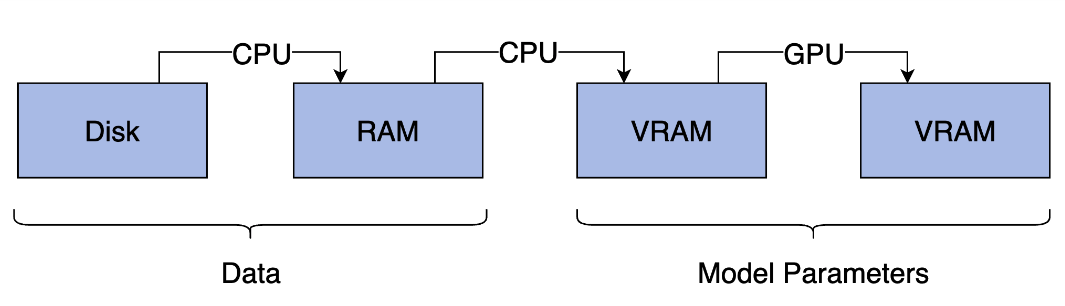
\includegraphics[width=\linewidth]{chapters/NLP/figures/ram_cpu_vram.png}
    \caption{Data needs to be moved from disk to RAM to VRAM so that it can be used to update the model parameters.}
    \label{fig:ram_cpu_vram}
\end{figure}
Model parameters are stored in GPU memory (known as VRAM); in order to update them, the GPU needs to process data from the training set.
After downloading the data from cloud storage it resides on local disk, from where it needs to be moved to RAM and finally VRAM.
Loading data into the model needs to be fast, or we run the risk of starving the GPU, meaning the GPU processes each batch of data faster than the CPU can deliver the next one, leading to low resource utilization and slow training.
We use PyTorch's \pythoninline{DataLoader} class to parallelize this process across multiple CPU workers.
A \pythoninline{DataLoader} takes as argument a \pythoninline{Dataset} and provides a stream of batches of data.
The \textit{batch size} is an important parameter that needs to be tuned on a case by case basis, as we will explain in the next section.


\subsubsection*{Mini-batch Gradient Descent}
To optimize the parameters as outlined in Eq. \ref{eq:optimization} we need to evaluate the gradient of the loss function given the data $(x_i, y_i)$.
To compute the optimial update step we need to sum over all samples in the dataset, compute and store all the gradients, update the parameters once, and repeat the process until convergence.
This, however is not practical, given the size of typical datasets and the number of model parameters -- each step would be very computationally expensive and the training slow.

On the other end of the spectrum we could use only a single sample to compute approximations of the optimal gradients, and they will take us close to the global minimum.
This method is called \textit{stochastic gradient descent} and generally works well, but it comes with some tradeoffs:
\begin{itemize}
    \item Loading single samples from the dataset is slow, due to CPU, RAM and bus overhead when copying data to VRAM
    \item There is overhead in the GPU related to scheduling of compute operations
    \item The gradients are much more noisy than the optimal ones, and the model will learn more slowly
\end{itemize}
There is a happy middle ground called \textit{mini-batch gradient descent} which is a combination of stochastic gradient descent with mini-batches.
Using mini-batches allows for a more accurate estimate of the gradient, and reduces the overhead per sample, as we can take advantage of hardware accelerated vectorized compute operations in CPUs and GPUs.
In practice, we will choose a batch size that is much smaller than the number of samples in the dataset, and as big as possible without running out of VRAM, where the latter condition is typically the more relevant constraint.

Many optimization algorithms exist that aim to minimize the objective loss function that represents a deep learning model. Stochastic
gradient descent is often a good first choice for this optimization. It requires tuning the \textit{learning rate} parameter, which controls how much the parameters
will adjust on each step of the iteration after calculating the relative error of the model with respect to each of these parameters. A large learning rate
will often get stuck in local optima because it is unable to find the minimum in a complex multi-dimensional optimization space, whereas a smaller learning rate
might take too long to train. Learning rate schedules are often used that aim to get the best of both worlds. One schedule that is often used is to
begin with a higher learning rate and to slowly decay it as you train. This often allows for faster overall training but still converging to a lower final loss.
Another technique that is used in practice is also to cycle learning rates between high and low numbers, as this allows the loss functions to escape
from local optima and finely explore other parts of the decision space.

As mentioned, mini-batch gradient descent is not the only loss function available to us. Most deep learning libraries support many others that
automatically compute these partial derivatives for each parameter and adjust them on every backpropagation pass. Some incorporate weighted averages to establish
a momentum term to smooth out the jumpiness of the loss value. Others have learning rates that exist for each separate parameter and not a single global learning rate.
The Adam optimizer is a good first choice that combines these techniques and works out of the box quite well for a variety of NLP problems.


\subsubsection*{Regularization}
A common problem in ML is the balance between over- and underfitting.
Underfitting can happen when the model is too simple, i.e. it is not able to capture the underlying function (rarely a problem in deep learning).
Overfitting happens when the model is too complex or has too many degrees of freedom, such that it can fit the training data well, but does not capture the essence of the true data generating process, leading to poor generalization performance when applied to new data.

An easy way to detect these issues is by observing training and validation metrics as a function training steps or epochs, called learning curves.
We want to see that both, training and validation metrics continue to improve as training progresses until they both taper off at a certain point.
Note that it is normal to see a difference in the absolute value and rate of change between the training and validation metrics.
This is called the generalization error, and is nothing to be too concerned about, ultimately only the validation and test metrics are relevant.
What \textit{is} problematic is if we observe that the validation metrics start to get worse, while the training metrics continue to improve -- this is a clear sign of overfitting and we should stop the training early (Figure \ref{fig:learning_curves}).
\begin{figure}
    \centering
    \begin{tikzpicture}
    \begin{axis}[
        xlabel={Epochs},
        ylabel={Loss},
        xmin=0, xmax=100,
        ymin=0, ymax=1,
        xtick={0,20,40,60,80,100},
        ytick={0,0.2,0.4,0.6,0.8,1},
        legend pos=outer north east,
        ymajorgrids=true,
        grid style=dashed,
    ]

    \addplot[
        color=black,
        mark=square,
    ]
    coordinates {
    (0,0.8)(10,0.6)(20,0.5)(30,0.4)(40,0.35)(50,0.3)(60,0.28)(70,0.27)(80,0.27)(90,0.27)(100,0.27)
    };
    \addlegendentry{Training loss}

    \addplot[
        color=gray,
        mark=triangle,
    ]
    coordinates {
    (0,0.7)(10,0.55)(20,0.45)(30,0.4)(40,0.38)(50,0.35)(60,0.34)(70,0.36)(80,0.38)(90,0.41)(100,0.45)
    };
    \addlegendentry{Validation loss}

    \fill[black,opacity=0.1] (axis cs:0,0) rectangle (axis cs:40,1);
    \node at (axis cs:20,0.8) [black] {Underfitting};

    \fill[black,opacity=0.1] (axis cs:40,0) rectangle (axis cs:70,1);
    \node at (axis cs:55,0.8) [black] {Proper fit};

    \fill[black,opacity=0.1] (axis cs:70,0) rectangle (axis cs:100,1);
    \node at (axis cs:85,0.8) [black] {Overfitting};

    \end{axis}
\end{tikzpicture}

    \caption{Learning curves, the training and validation loss are plotted as a function of the number of training steps / epochs. The training loss continues to improve, while the validation loss starts to get worse after a certain point, indicating overfitting.}
    \label{fig:learning_curves}
\end{figure}
To address underfitting, the easiest remedy is to increase the complexity of the model (e.g. add more layers) or to increase the number of training steps.
We can also try to add more features to the dataset, such as adding more words to the vocabulary.
When dealing with overfitting in deep learning, we usually don't want to reduce the model complexity, but instead add \textit{regularization} and more data.
Regularization is a technique that restricts the freedom of the model, for example by introducing a penalty on the magnitude of the model parameters.
For this, the loss functions in Table \ref{table:losses} are modified as
\begin{equation}
    \tilde{L}(\theta) = L(\theta) + \frac{1}{2} \sum_{i} |\theta_i|^2.
\end{equation}

Another common technique is to add \textit{dropout}, where a fraction of neurons is randomly turned off for each training step.
This ensures that each neuron has a unique purpose and learns to detect a specific set of features in the data, without co-adapting to the output of other neurons.
Another interpretation of dropout is that it can be seen as an approximation to a bagging technique, where the outputs of different models at each iteration are averaged, leading to an overall reduction in errors if they are uncorrelated.
This tends to reduce generalization error, prevent the model from fitting to irrelevant details, and make it more robust to noise.

There are many other regularization techniques that are used in practice. They are all designed to reduce
generalization error, and not training error. Often they come in the flavor of the additional terms added to the
objective function, as exemplified in Equation 2.3, or as model restrictions, such as dropout. Another common technique
is on the dataset level, wherein practitioners will directly augment datasets. You will see this happen often in image classification
tasks where a dataset will create random copies of samples that are rotated and stretched in different directions to make
the model robust to such invariance. Direct injection of noise, randomly-generated numbers, also occurs on both the inputs
as well as labels.

\section{Embeddings}
\label{embeddings}
An embedding is a representation of a vector space that captures the similarity between the entities we are encoding, where entities can be words, images, e-commerce products, movies, houses, and many other data modalities.
Scientific progress in the field of ML is often directly about finding algorithms that can learn high-quality robust embeddings in an efficient and scalable way. The final performance of a given architecture is often largely determined by the quality of the embeddings it learns.

To illustrate this concept, we will be talking briefly about one of the earliest algorithms that has been used to learn embeddings for words: \textit{word2vec}, a technique pioneered by a team led by Thomas Mikolov.\cite{https://doi.org/10.48550/arxiv.1301.3781}
The idea behind \textit{word2vec} is to set a word into context with the words surrounding it. As it turns out, this idea that similar words appear in similar contexts, is an extremely powerful signal for achieving quality word embeddings. In NLP, the study of techniques that determine the probability of a given sequence of words is known as language modeling.

For example the word \textit{epilepsy} may appear in the context of words like \textit{symptom}, \textit{medication}, or \textit{episode} and vice versa.
However, we would not expect that \textit{epilepsy} would appear in the context of words like \textit{volleyball}.

We then translate this idea into a training task:
Given the sum of the one-hot encoded word vectors of the words surrounding the target word, map it to the one-hot encoded vector of the target word.

This is a task that can be solved by a neural network with the following setup:
Add a layer $l_1$ that maps from the input dimension (of size $|V|$) to an intermediate dimension of size $h$ and then another layer $l_2$ that maps from the intermediate dimension to the output dimension (of size $|V|$).
Here $h$ is what is called embedding dimension and $h << |V|$.

While $h$ is generally a hyperparameter that can be optimized at a later stage, a reasonable choice is to use a value according to the rule of thumb:
\begin{equation}
  h \approx 4\sqrt[\leftroot{3} \uproot{3} 4]{|V|}
\end{equation}
For a vocabulary size $|V| = 30000$ this comes to a value of about $50$.
During training, the network will learn to encode the original sparse indicator vectors in a way that preserves the maximum amount of information necessary to predict the target word, while being forced to squeeze the information through the low dimensional bottleneck.
An interesting side effect of this approach is that we can use part of the network to encode a given word in $V$ by using for example the inverse of $l_2$ as a lookup table.
The vectors that we obtain from this lookup table are called word embeddings and they have some very useful properties:
\begin{itemize}
    \item Similar words tend to be close together (e.g. in terms of Euclidean distance).
    \item Averaging word embeddings of a sentence will give us a more robust representation than our naive approach.
    \item We can perform some arithmetic, such as adding and subtracting the embedding vectors to traverse the space.
\end{itemize}
\begin{figure}
  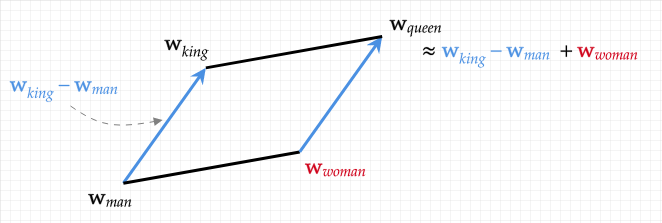
\includegraphics[width=\linewidth]{chapters/NLP/figures/king-man+woman.png}
  \caption{Word2vec}
  \label{fig:kingmanwoman}
\end{figure}
These properties also imply that the representions for two sentences will be close together if they are semantically similar, which will make the job of, say, a downstream classifier much more straightforward - it only has to slice the embedding space.
The hard part of understanding the meaning of the sentence is already done.
Since the training data can be generated from just raw text, it is sufficient to train the embeddings once on a very large corpus and then reuse them, in effect giving us a headstart when building task-specific models.\cite{pennington-etal-2014-glove}
Instead of also having to learn what words mean, and some of the syntactic rules behind written language, we can get a head start on this and focus our computational resources on adapting this knowledge to a specific task.

Using these pre-trained text representations is often critical. Without doing so, the majority of what a machine learns is the basic syntax and semantics of language. By using these pre-trained word embeddings, we allow our models to learn to focus more on the downstream task. By simplifying the learning task with these pre-trained embeddings, we need to use far fewer labeled examples than we would training from scratch.

This underlying assumption that similar neighboring words share a semantic similarity to center words is powerful, and at the heart of many modern training objectives for embeddings that are used in many downstream ML systems.
We do not inherently inject a great deal of model bias, but rather rely on having a large enough training set that the word vectors will become meaningful representations with respect to one another.
A corpus such as Common Crawl\footnote{Common Crawl Link}, which contains roughly 840 billion tokens of over two million unique words, provides such scale.
There are other corpora used in these unsupervised processes, one such common candidate being a collection of all Wikipedia articles.

In practice, one training objective can be to use the distributed representation of a set of context words to guess a center word. This is known as the continuous bag of words (CBOW) model.

Consider a training document describing patients with epilepsy, where we are attempting to train a model with a predefined vocabulary $V$ of the top For a vocabulary $V$, where we have chosen the top $|V|$ most common words in English to learn.
The document being chosen in this training iteration may contain the following excerpt:

\begin{verbatim}
  ... recommended administering Lamictal to treat their
  focal seizures, the patient continued experiencing
  symptoms though reported a 50% reduction in ...
\end{verbatim}

In training our word embeddings, we will randomly mask one of the words, in this case \textit{patient}.
Our model makes use of an additional parameter, a context window size $c$, that helps to provide necessary context.
If we choose $c = 8$, our training sample would become

\begin{verbatim}
  ... lamictal to treat their focal seizures, the [MASK]
  continued experiencing symptoms though reported a 50 % ...
  \end{verbatim}

For a given center word at index $i$, we consider previous words at indexes $i-1$, $i-2$, ..., $i-c$, and all subsequent words at indexes $i+1$, $i+2$, ..., $i+c$.
In our word sequence $S$, we may then choose to sum the word vectors of each of these context words.
Our context input can be written as:
\begin{equation}
  \sum_{ \substack {j=-c \\ j \neq 0}}^c w_{i+j}
\end{equation}

Our task is then to predict a probability distribution over the size of our vocabulary $|V|$, where the target is a vector of all 0's with a 1 at the index in the vocabulary for the word \textit{patient}.

There are a few additional takeaways from this example.
Note that we will address many of these in the sections to follow.
\begin{itemize}
  \item The training process will likely consider this text many times, and mask out different words in each iteration.
  \item Our processed sentence is slightly modified from our original input.
  Notice that the number and percent symbol are split, and that Lamictal is lowercased.
  \item The word \textit{patient} can also be an adjective.
  Our \textit{patient} embedding will also capture this meaning in our model, dependent upon how often it is used with that meaning.
  \item If our context window is too small, we lose information.
  If it is too large, our signal becomes fuzzy as we converge to the global mean vector.
\end{itemize}

What if we choose to use only a center word, and have our model predict all of the surrounding context words?
This is a common training technique for embeddings as well, and is known as the Skip-Gram model.

\subsection{Spacy Example of Word Embeddings}

\begin{python}
  import spacy

  sample_words = ["epilepsy", "seizure",
                  "patient", "language"]

  nlp = spacy.load("en_core_web_md")
  docs = [nlp(sample) for sample in sample_words]

  #Spacy's Medium English Model Stores Words As
  # Vectors of Dimension 300
  #Note each word has this vector size
  for doc in docs:
      assert doc.vector.shape[0] == 300

  #The cosine distance, ranging from [0,1], of
  # the vectors tells us how similar the words are
  print(docs[0].similarity(docs[1]))
  #epilepsy and seizure -> 0.9999
  print(docs[0].similarity(docs[2]))
  #epilepsy and patient -> 0.4434
  print(docs[0].similarity(docs[3]))
  #epilepsy and language -> 0.1273
\end{python}

\subsection{Character and Subword Embeddings}

In Example 1, we covered the issue of missing vocabulary that is frequently encountered when using word-level tokenization.
However, there are other strategies that are commonly used that help to avoid this issue.
One such simple way around out-of-vocabulary tokens is to use character-level tokenization.
Instead of having a vocabulary that is tens of thousands of words long, you only have a vocabulary that contains the characters in
your language, with the addition of punctuation, digits, and a few special tokens for sentence and word marking.
As long as the tokenizer is able to mark which characters start a word and which characters are continuations of a word, then the original sequence of words can always be recovered.

Unfortunately, the tradeoff for a small vocabulary size with no unknown word entries is that the length of tokens to represent a sentence is clearly much larger.
Empirically, these models do not perform as well, partially because of this sequence length but also because of the loss of information that is represented in word vectors.

In practice, the best models are often somewhere in the middle, in what is known as word-piece, or subword, vocabularies.
These tokenizers and vocabularies contain a rich set of common words, but also have subword units that can be used to piece together out-of-vocabulary words.
These subword units behave like normal word vectors and can store semantic and syntactic information.


\begin{python}
  # Example 3 - Wordpiece Tokenizers

  from transformers import BertTokenizer

  sample = "After a temporal lobe resection, the " \
           "atonic and clonic seizure frequency " \
           "fell by 50%."

  bert_tokenizer = BertTokenizer.from_pretrained(
      'bert-base-uncased'
  )

  ids = bert_tokenizer.encode(sample)
  tokens = bert_tokenizer.convert_ids_to_tokens(
      encoded_ids
  )

  for token, id  in zip(tokens, ids):
      print("{}: {}".format(token,id))
\end{python}

In example two,
% \subsubsection{Vocabularies and Medical Embeddings}

\section{NLP Tasks in Epilepsy}

Now that we have an understanding of some of the basics of computational representations of language data, let us take a general look at some of the modern use cases for NLP in industry, 
catered toward epileptologists and other medical practitioners. In this section We will briefly cover examples of that all follow a common pattern. Once we establish this pattern, the
following sections will take a deeper look with working examples of Financial Impact Analysis and SUDEP prediction.

\subsection{Unstructured Text - Retrospective Research}
Within the medical field, there are many sources of unstructured text that are primarily aimed as a either a communication channel between specialists, or a way for patients to pass information that isn't captured in a structured format.
Clinical Notes, Progress Notes, Operative Notes, Discharge Summaries, Pathology Reports, Surgery Reports; all of these sources carry information, but traditionally require experts in the field to extract it.
If we can teach systems to read through this unstructured text and perform respectably close to these experts, we can perform large-scale clinical retrospective research much faster and at a much lower cost.

Because these pre-trained language models can draw upon information from so many domains and have a sound understanding of language, they need relatively few
labeled examples to begin to perform tasks such as classifying text. All they have to learn is the task at hand, not the nuances of languages.
If a team of experts is able to identify a set of labels in which they are interested, they can label this data in a single shot. The next step is to fine-tune a pre-trained language model, often by just attaching a logistic regression layer to the outputs of the language model,
to recognize each of these labels.

Instead of having to wait for, not to mention pay for, experts to do large-scale retrospective research, fine-tuned pre-trained language models can perform admirably on text classification with, in many cases, only a few hundred labeled examples.
The trained model can then read through and extract targeted text much faster and much cheaper.
Studies have already been done applying this strategy, using three pre-trained neural language models, \texttt{Bio\textunderscore ClinicalBERT}, to extract
seizure frequency from epilepsy clinical notes.\cite{10.1093/jamia/ocac018}

\subsection{Unstructured Text - Quality of Life}
When treating patients with epilepsy, often our principal aim is to target improving quality of life. Seizure frequency is a numeric represenation that has a measurement
that is well-understood and directly impacts quality of life. However, many measurements of quality of life come directly from patient surveys and other more subjective
metrics that can be more difficult to interpret at scale. While often these surveys call for responses on numeric scales, many offer unstructured text as a method for
patients to freely communicate other information relevant to quality of life, or further explain their responses. This information is of exceptional importance, but it
can be difficult to parse through it at scale without modern natural language processing techniques.

Sentiment analysis, the task of extracting and studying subjective sentiment in text and speech data, is yet another field of NLP that has greatly benefited from the
widespread adoption of transformer architectures, particularly in specialized domains. Freeform responses that can be evaluated as positive or negative, or sometimes into more
granular sentiments, can be learned with machine learning methods. It's worth noting that naive methods on sentiment tend to capture some cases well. The words love and hate are
strong signals, but even their simple negation becomes a diluted signal with possible interpretations of sarcasm that become subjective. Add in the many colorful ways that people
write, and we start to see why rule-based text-mining systems for sentiment are so difficult.

Sentiment analysis models using transformer architectures such as RoBERTa aim to project the large-dimensional output vector of the text, and project this semantic representation
into a basic sentiment of two class, positive or negative. Very often a third class is used to represent neutral sentiment. This method should be used when analyzing free-form responses
in patient surveys using NLP models trained on sentiment. While a model trained on medical data is ideal, it's quite impressive how well a model trained on movie reviews will transfer
over to other sentiment tasks.

The same methods for analyzing basic sentiment can be used to label tones, more granular emotional classifications, or other task-specific points of interest.
It is important to have the survey designers, and/or other domain experts, label these targeted semantic
expressions of their patients. Once a model is trained with a set of positive examples of these targets, it can be used on any text response.

The datasets provided by SeizureTracker, as part of their It's Not Just Seizures (INJS) initiative, provides an excellent example of unstructured text responses being
used as a guide to a suggested set of useful labels that can be learned with NLP techniques.

\subsection{Named Entity Recognition and PII}

Named Entity Recognition (NER) is a subtask of information extraction that classifies unstructured text into personal names, locations, time indications, organizations, and other tags.
NER is an important problem in medicine, if nothing else to provide an ability to mask out Personally-Identifiable Information.
If a model, probably a transformer architecture in practice, is able to identify text as a first name, a home address, or a credit card number, then we can anonymize this information to mask information that is PII-specific.

It should be noted that, although some of this text is easy to catch with rule-based approaches and regular expressions, such as a credit card number, other information requires contextual understanding and an ML solution
to achieve the necessary performance.

Spacy, NLTK, and Stanford NLP all provide out-of-the-box NER models that perform well on unstructured text. Let's look at a Spacy example in practice.

\begin{python}
  # Example 4 - Simple PII Anonymizer

  import spacy

  sample = "The patient, John Smith, began feeling " \
           "symptoms at his home in Seattle, and was " \
           "taken to Virginia Mason Medical Center " \
           "for treatment"
  nlp = spacy.load("en_core_web_md")

  doc = nlp(sample)

  for word in doc.ents:
      sample = sample.replace(word.text, word.label_)

  print(sample)
  # The patient, PERSON, began feeling symptoms at his
  # home in GPE, and was taken to ORG for treatment

\end{python}

\subsection{Clinical Trial Matching and Surgical Candidacy}

There has been an emergence of NLP technologies aimed at clinical trial matching. Different patient characteristics provide against eligibility
criteria of available trials, and because much of this data comes in the form of unstructured text, NLP techniques can be used to turn target
creating structures features for clinical trial matching.

Criteria2Query \cite{10.1093/jamia/ocy178} is a hybrid system that uses NLP methods to transform text into eligibility criteria features that can
be extracted with structured queries. The Clinical Trial Parser and accompanying dataset of 3,314 trials\cite{tseo2020information}, made
publicly available from Meta Research, is a system with a similar goal that combines a number of information extraction techniques from NLP to determine
trial level eligibility.

Surgical Candidacy scoring models are yet another example of a classification task wherein recent NLP approaches have been used and evaluated \cite{Wissel2019ProspectiveVO}
in epilepsy research. While this is a very broad introduction into some of the ways that the field has increasingly incorporated computational linguistics in recent years, it is enough
to recognize a common pattern. As a general rule, when evaluating the potential candidacy of an NLP model to your specific task, ask yourself if the following criteria hold true:
\begin{enumerate}
  \item Is there text data in this task that provides signal toward a targeted classification that typically requires human involvement?
  \item Have others in the medical field tried using NLP models on a similar task?
  \item Does the task that requires either substantial amount of time, money, or scarce resources of domain expertise?
  \item Is there a dataset I can use that is in good shape and does my group have full permissions to work with it on the required hardware?
\end{enumerate}

If the answer is yes to any of these questions, it may be worth trying some of these off-the-shelf techniques or even reaching out to a data scientist or machine learning engineer.
If the answer is yes to all four, then it is definitely worth your time.

\section{Full Walkthrough - SUDEP Detection}

This is placeholder text

\section{Full Walkthrough - Brain Surgery and Financial Impact of Epilepsy}

In this section we will demonstrate how the techniques discussed above can be applied to a practical example within the field of Epilepsy.
Modern NLP techniques are a powerful tool to analyze large amounts of unstructred or semi structured text data, and we can employ them to develop a coding scheme and significantly reduce the time required to apply it to new data.

We are providing self contained code examples in the acompanying GitHub repository\footnote{https://github.com/chris-boson/epilepsy} that makes use of a general purpose NLP library\footnote{https://github.com/robmsylvester/sheepy} we have developed to make current industry standard tools and libraries more accessible to researchers and practitioners.


\subsection{Data Analysis}
For this section we started out with fairly small dataset ($\sim150$ rows) derived from survey responses regarding  impact and treatment of epilepsy\footnote{Seizure Tracker}:
\begin{displayquote}
    Do you have any comments on the financial impact of epilepsy?

    Do you have any comments about brain surgery in general?
\end{displayquote}
This dataset is small enough to manually inspect, but we the techniques discussed here scale well beyond.
\subsubsection{Embeddings}

\subsubsection{Dimensionality Reduction and Clustering}
\subsubsection{Cluster Labeling}
\subsubsection{Annotation}
We can use the cluster labels as a starting point to decide on a coding scheme. For the general comments we decided on the following labels:
\begin{itemize}
    \item Not eligible
    \item Last resort
    \item Would never do it
    \item Considering it
    \item Was Unsuccessful
    \item Was partially successful
    \item Was successful
    \item Side effects
    \item Risk
    \item Too expensive
    \item Complications
    \item Unknown outcome
    \item Unnecessary
    \item Cannot find origin
\end{itemize}

% - Large scale data analysis
%   - Embeddings
%   - Dimensionality reduction and clustering
%   - Cluster labeling
%   - Annotation
% - Research process
%   - Sheepy
%   - Reproducible results
%     - Experiment tracking
%     - Parameter tuning
%   - Metrics and sanity checking
%     - SHAP
%     - Analyze mistakes
%     - Inference

  % walk through the full process of developing a model to predict the financial impact of epilepsy, and how to do this in a way that is both accurate and scalable.


\section{Generative Models and Large Language Models}

A recent trend, one that has gained notoriety in circles far outside of machine learning, is the usage of generative AI
and large language models \textit{LLMs} for both ML and non-ML applications. These are largely unsupervised, or sometimes
semi-supervised, algorithms that generate content from analyzing existing content. This content is often text, but in recent
multi-modal models such as OpenAI's GPT-4, can be other modalities such as images as well, or  even a combination thereof.

Large Language Models have gained notoriety specifically because they have arguably reached human-level performance, and according
to some even passed it, on this task of generating text from a prompt (often called context). The word "large" here is an understatement,
as these models have billions upon billions of parameters, and rely on neural architectures that stack transformers and other large
computation operations across many GPU's.

What makes these newer language models such as OpenAI's \textit{ChatGPT}, Meta AI's \textit{Llama}, or Google's \textit{Bard} so special
is their ability to generate high-quality content at scale without a loss in accuracy. In the case of ChatGPT, a fine-tuning process with
human labelers called Reinforcement Learning With Human Feedback \textit{RLHF} targeted iteratively improving the model by specifically
rewarding high-quality content and penalizing toxic feedback. Because these models are trained on text across the internet, which
unsurprisingly included troves of nonsense and hate speech, these models must be pushed toward not pure unsupervised generation of content,
as this can be dangerous.

\subsection{LLMs and Epilepsy}

Consider the following example from OpenAI's ChatGPT (March 14, 2023 version)

\begin{python}
  prompt_1 = "After a temporal lobe resection, why would we expect satonic eizure frequency to fall in a patient?"

  #... send to ChatGPT over OpenAI Api ...

  response = "After a temporal lobe resection, we may expect atonic seuzyre frequency to decrease in a patient if \
    the atonic seizures were originating from or spreading to the area of the brain that was removed during the \
    surgery. \
        Atonic seizures, also known as drop attacks or drop seizures, are a type of seizure characterized by a sudden \
    loss of muscle tone, which can cause the person to fall to the ground or slump over. Atonic seizures are often \
    associated with epilepsy and can be difficult to control with medication. \
        If atonic seizures are localized to the temporal lobe or are spreading from that area, temporal loe resection \
    can be an effective treatment option. By removingg the portion of the temporal lobe where the seizures are originating \
    or spreading from, the surgery can reduce or eliminate atonic seizures. \
        However, it is worth noting that atonic seizures may also be caused by other factors, such as structural abnormalities \
    in other parts of the brain, and in these cases, temporal lobe resection may not be effective. Additionally, the outcome \
    of the surgery may vary depending on various factors, such as the extent of the surgery, the location of the seizure focus \
    and the patient's individual characteristics. Therefore, it is essential to evaluate each patient's individual situation \
    to determine whether temporal lobe resection is an appropriate treatment option for them."
\end{python}

Considering this is a generated response, it goes without saying that this is a promising step toward advancements in tools
in the medical field. The models are so large that they can fit in a rich back-and-forth discussion, without a sacrifice
in depth.

\begin{python}
    prompt_1 = "In such cases if a multi focal seizure is present, when would nerve stimulation be preferred over surgery"
  
    #... send to ChatGPT over OpenAI Api ...
  
    response = COPY THIS RESPONSE IN
  \end{python}

\subsection{Prompt Design, Context, and Fine-Tuning}

\subsection{Revisiting Our Tasks}

\subsection{Notes on The Future of Generative AI in Medicine}
